\section{Analisa}
	Pada subbab ini, penulis akan memaparkan analisa-analisa kebutuhan, teknis dan analisa pribadi serta pengaruhnya dalam perancangan aplikasi pada subbab \ref{perancangan-sistem}. Secara garis besar, subbab ini menjelaskan \begin{inlinelist}
		\item analisa kebutuhan fungsional,
		\item analisa aspek bisnis,
		\item spesifikasi kebutuhan, dan
		\item rancangan arsitektur dan teknologi yang digunakan
	\end{inlinelist}. Pada beberapa poin, penulis akan menyertakan rancangan dan pemilihan teknologi yang berdampak dari hasil analisa tersebut.
	
	%Requirement Analysis
	\subsection{\textit{Requirement Analysis}}
	
	
	\subsubsection{Fungsionalitas Dasar}

Aplikasi Lelang Online berbasis Web yang diberi nama \textbf{Lelangapa} adalah sebuah \textit{online auction web} yang dibangun berdasarkan paper rujukan utama, dengan fitur-fitur utama sebagai berikut:

\begin{enumerate}
	\item \textbf{Registrasi ke dalam sistem}
	\item \textbf{Login ke dalam sistem}
	\item \textbf{Mendaftarkan barang untuk dilelang} \\
	Pengguna dapat mendaftarkan barangnya untuk dijual dan dilelang. Selain itu, pengguna dapat menentukan harga awal dan batas waktu lelang pada saat mendaftarkan barangnya.
	\item \textbf{Memperbarui barang yang dilelang} \\
	Pengguna dapat memperbarui informasi mengenai barang yang dilelang, seperti nama barang, menambah foto deskripsi barang, atau menambah waktu lelang.
	\item \textbf{Melihat informasi barang yang dilelang} \\
	Pengguna dapat melihat detail informasi barang yang sedang dilelang – seperti foto barang, riwayat penawaran harga barang lelang, sisa waktu penawaran, deskripsi barang, dsb.
	\item \textbf{Melihat informasi riwayat lelang} ( Siapa saja yang sudah mengajukan penawaran dan harga yang ditawarkan )
	\item \textbf{Mengajukan penawaran harga untuk barang yang dilelang / Menjadi auctioneer} \\
	Selain menjadi auctioneer, pengguna juga dapat menawarkan harga terhadap barang-barang yang didaftarkan oleh pengguna lain.
	\item \textbf{Mendapatkan pemberitahuan jika penawaran harga dikalahkan dengan harga lebih tinggi} \\
	Pengguna mendapatkan pemberitahuan jika pengguna sedang mengikuti pelelangan barang, dan ada penawaran harga yang lebih tinggi dari penawaran oleh pengguna tersebut, sehingga pengguna dapat mengikuti perkembangan harga dari barang yang dilelang.
	\item \textbf{Mengikuti / follow barang yang sedang dilelang dan mendapatkan pemberitahuan jika barang tersebut }\\
	Jika pengguna sedang tidak ingin melelang barang namun ingin tetap mengetahui informasi dari suatu barang lelang, pengguna dapat mengikuti feed/berita dari barang tersebut.
	\item \textbf{Mendapatkan pemberitahuan jika memenangkan lelang atau tidak.}\\
	Jika pengguna mengajukan penawaran harga terhadap suatu barang, maka pengguna akan mendapatkan pemberitahuan pada saat batas waktu lelang selesai, apakah pengguna tersebut memenangkan proses lelang tersebut atau tidak.
	\item \textbf{Saling berkirim pesan singkat/chat kepada auctioneer/penawar harga }\\
	Untuk saling bertukar informasi mengenai barang yang sedang dilelang, auctioneer dan penawar harga dapat saling berkirim pesan singkat.
	\item \textbf{Melihat riwayat penawaran harga lelang }\\
	Pengguna dapat melihat barang riwayat penawaran harga yang diberikan oleh pengguna tersebut terhadap semua barang yang pernah dia lelang.
	\item \textbf{Melihat riwayat barang yang dilelang }\\
	Pengguna dapat melihat riwayat barang yang pernah ditawar harganya/diberikan penawaran harga.
	\item \textbf{Memberi review tentang pengguna lain sebagai auctioneer dan atau sebagai penawar harga }\\
	Pengguna dapat memberikan komentar/testimoni berdasarkan pengalaman bertransaksi/penawaran harga dengan pengguna lainnya, baik pengalaman memuaskan ataupun pengalaman buruk.
	\item\textbf{ Melihat review mengenai seorang pengguna }\\
	Selain memberikan review, pengguna dapat melihat review seorang pengguna.
	\item \textbf{Memblok pengguna sebagai auctioneer }\\
	Auctioneer dapat memblok pengguna agar pengguna tersebut tidak memberikan penawaran harga terhadap barang yang sedang ia lelang. Hal ini bisa saja karena review/testimoni pengguna tersebut buruk atau karena alasan lainnya.
	\item \textbf{Mencari barang yang dilelang dengan keyword tertentu}
\end{enumerate} %checked
	
    \subsubsection{Analisa Paper Rujukan}
	    \label{analisa-paper-rujukan}
	    Dengan perkembangan teknologi, perlahan kebiasaan manusia berubah. Termasuk juga dalam perdagangan, dimana transaksi jual beli barang tidak lagi harus melalui tatap muka. Penjualan online saat ini sudah dapat dilakukan lewat berbagai cara, antara lain menggunakan e-commerce, atau posting di social media, atau bisa juga dengan melelang di aplikasi lelang online. Sedikit berbeda dengan teknik penjualan di lelang online, karena aplikasi ini dapat diakses oleh banyak orang, tentu saja pelelang (\textit{auctioneer}) tidak terbatas pada ruang lelang saja, tapi bisa berasal dari manapun selama mereka mengakses aplikasi tersebut.  Lelang online ini tentu saja mendatangkan banyak manfaat, selain biaya yang lebih efisien dan hemat, dan juga tidak menguras waktu karena siapapun, kapanpun, dimanapun dapat mengajukan penawaran ataupun melelang barangnya tanpa harus pergi ke instansi tertentu dan melakukan lelang dengan cara konvensional.\\
		\indent Bercermin terhadap aplikasi \textit{e-commerce} yang telah ada, masalah yang paling sering dialami adalah ketidakpuasan pengguna. Salah satu indikator bahwa suatu perusahaan dikatakan memiliki ketidakpuasan pelanggan adalah karena kegagalan dalam pelayanannya. Seorang pelanggan sangat mungkin memutuskan untuk komplain setelah mengalami ketidakpuasan terhadap layanan suatu perusahaan, dan jika tidak ditangani dengan baik, hal ini bisa berakibat fatal terhadap reputasi dan kepercayaan pengguna terhadap aplikasi tersebut. \\
		\indent Oleh karena itu, sebuah paper mengangkat topik ini khusus dalam bidang aplikasi lelang online, menganalisa kegagalan dan ketidakpuasan pengguna, beserta solusi-solusi yang ditawarkan oleh pengguna aplikasi untuk memperbaiki kegagalan pelayanan tersebut. 
		
	  \begin{figure}[H]
        \centering
        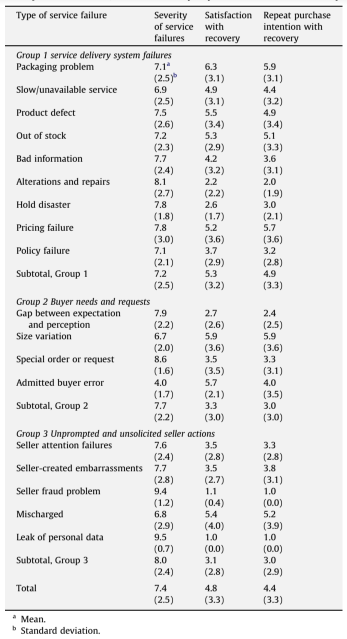
\includegraphics[height=.5\textheight]{images/bab3/Fatalitas-Kegagalan-Ecommerce.png}
        \caption{Fatalitas kegagalan dalam aplikasi Lelang Online, Kepuasan terhadap Perbaikan Pelayanan dan \textit{Repeat Purchase Intention} setelah Perbaikan Layanan}
        \label{severity-failures}
      \end{figure}
      
      \indent Dalam gambar diatas, dijabarkan beberapa jenis kegagalan yang pernah dialami oleh pengguna aplikasi serta fatalitas/pengaruh buruk kegagalan tersebut terhadap kepercayaan pengguna. 
      
	  \begin{figure}[H]
        \centering
        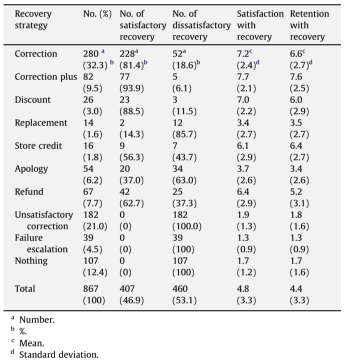
\includegraphics[width=\linewidth]{images/bab3/Solusi-Perbaikan-Ketidakpuasan.png}
        \caption{Kategori Perbaikan terhadap Kegagalan Pelayanan Lelang Online}
        \label{service-recovery-strategies}
      \end{figure}
      
      \indent Maka berdasarkan hasil analisa tersebut, fitur-fitur yang perlu ditambahkan selain daripada fitur dasar aplikasi lelang online adalah sebagai berikut :
      \begin{enumerate}
      \item Fitur chatting, untuk mengurangi kemungkinan \textit{Bad Information} dimana ekspektasi dan persepsi terhadap barang yang dilelang antara pembeli dan penjual tidak sama dan \textit{Special Needs}, 
      \item Fitur pemberian kupon voucher (\textit{Discount and Correction Plus}) yang bisa berupa \textit{free shipping} atau \textit{discount}.
      \end{enumerate}
   %checked
	\subsection{\textit{Bussiness Aspects of Software Engineering}}
	
	Lelang merupakan salah satu metode pertukaran barang dan jasa dengan metode penetapan harga yang berbeda dengan perdagangan. Oleh karena itu, lelang juga termasuk dalam kategori bisnis. Yang menarik adalah, ketika bisnis digabungkan dengan teknologi atau yang sering disebut \textit{e-commerce}, hal yang sekedar pertukaran barang bertransformasi menjadi sebuah sistem interaktif yang kompleks dimana tujuan utamanya adalah menarik pengunjung/pengguna untuk menyelesaikan sebuah transaksi. Hal ini tentu sangat krusial, penting, dan tertantang untuk menyelesaikannya. \\
	\indent Dalam mencapai kesuksesan dan tingkat kompetitif yang tinggi, haruslah menyediakan layanan dengan kesan \textit{user experience (UX)} yang positif bagi para penggunanya. Morville  \cite[p.~27]{a-set-of-heuristics-2014} , dalam studi yang dilakukannya, menyebutkan bahwa UX tercakup dalam 7 aspek esensial, yaitu \begin{enumerate}[label=\alph*.]
		\item \textit{useful}
		\item \textit{usable}
		\item \textit{findable}
		\item \textit{desirable}
		\item \textit{accessible}
		\item \textit{credible}.
		\end{enumerate}
	
	\indent Hasil-hasil temuan penting yang menarik dalam pengaruh \textit{user experience}, adalah sebagai berikut dikutip dari sebuah sumber adalah sebagai berikut:
	\begin{enumerate}[label=\alph*.]
		\item \textit{User tend to leave if a page loads more than 3 seconds};
		\item \textit{79\% of users won't return if the web's performance and experience is poor};
		\item \textit{44\% of users will tell the poor experiences to their friends}.
	\end{enumerate}
	
	\indent Selain dari faktor \textit{user experience} dan \textit{performance}, beberapa hal yang menjadi poin penting dan menarik dalam beberapa studi yang terkait adalah sebagai berikut:
	\begin{enumerate}[label=\alph*]
		\item \textit{Familiarity} - yang dapat didefinisikan sebagai tingkat familier atau kesamaan dengan sistem sejenis ternyata dapat membangun \textit{trust} sehingga mensugesti pengguna untuk menyelesaikan transaksi yang dilakukan;
		\item \textit{Usability} yang memudahkan pengguna dalam menyelesaikan transaksi; dan
		\item Aspek-aspek psikologi seperti pemilihan warna, penggunaan \textit{icon} yang sesuai, seperti \textit{icon} gembok pada halaman pembayaran ternyata dapat mengesankan \textit{security} pada pengguna.
	\end{enumerate}
	
	
	\begin{figure}[H]
		\centering
		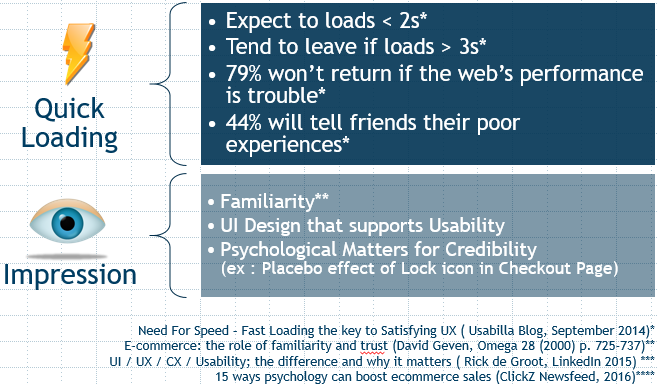
\includegraphics
		[width=\textwidth]
		{images/bab3/analisa/user-centered.png}
		\caption{Visualisasi aspek bisnis dalam \textit{software engineering}}
		\label{user-centered-analysis}
	\end{figure}
	
	\indent Dari hasil temuan ini, dapat disimpulkan bahwa \textit{user experiences, performances, usability} dan psikologi memiliki pengaruh besar dalam kesuksesan lelang online dalam menarik hati para penggunanya. Hal ini akan mempengaruhi definisi kebutuhan fungsionalitas yang akan dibahas dalam subbab \ref{keb-fungsional}.
		
		
		 
	  \subsubsection{Spesifikasi Kebutuhan Fungsional}
  \label{keb-fungsional}
	Berdasarkan deskripsi umum sistem pada subbab \ref{deskripsi-umum-app}, maka dapat disimpulkan bahwa kebutuhan fungsional dari aplikasi lelang online, yang dipaparkan dalam Tabel \ref{tabel-fungsional}.

  \LTXtable{\textwidth}{tables/03b/functional.tex}	
   %checked
	
  \subsection{Spesifikasi Kebutuhan Non-Fungsional}
  
  Kebutuhan non-fungsional yang harus dipeuhi oleh aplikasi ini berhubungan dengan faktor-faktor sebagai berikut:

	\LTXtable{\textwidth}{tables/03b/nonfunctional.tex}	
  
  \newpage %checked
	\subsubsection{\textit{Bussiness Modelling Workflow}} 
	\subsection{Spesifikasi Kasus Penggunaan}
	Kasus penggunaan disini dimaksudkan untuk menurunkan kebutuhan fungsional yang telah dispesifikasikan sebelumnya pada tabel \ref{tabel-fungsional} sebelumnya.\\
	Daftar kasus Penggunaan dapat dilihat pada \ref{kasus-penggunaan}.
	
	\LTXtable{\textwidth}{tables/03c/kasus_penggunaan.tex}
	\begin{figure}[H]
		\centering
		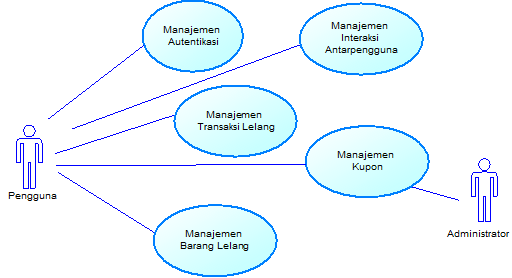
\includegraphics
		[width=\textwidth]
		{images/bab3/usecasediagram/ucd-main.png}
		\caption{Diagram Kasus Penggunaan Aplikasi}
		\label{ucd.main}
	\end{figure}
	
	Selanjutnya, akan dijabarkan masing-masing Spesifikasi Kasus Penggunaan untuk semua  Kasus Penggunaan yang telah dijabarkan diatas.
	
	\subsubsection{KP01. Manajemen Authentikasi Pengguna}

	Pada kasus penggunaan ini, pengguna dapat memanajemen autentikasi dan pendaftaran ke dalam sistem.\\

	% Login
	\begin{table}[H]
	\centering
\begin{tabular}{|r|p{8cm}|}
		\hline
		\textbf{Kode}                                                    & UC-01.01                                                     \\ \hline
		\textbf{Nama}                                                    & \textbf{Registrasi}                                         \\ \hline
		\textbf{Aktor}                                                   & Pengguna                                                    \\ \hline
		\textbf{Deskripsi}                                               & Pengguna mendaftar ke dalam akun agar masuk ke dalam sistem \\ \hline
		\textbf{Tipe}                                                    & Fungsional                                                  \\ \hline
		\textbf{\textit{Precondition}}
			& Pengguna belum memiliki akun di aplikasi                    \\ \hline
		\textbf{\textit{Postcondition}} 
			& Pengguna sudah memiliki akun terdaftar di aplikasi          \\ \hline
		\multicolumn{2}{|c|}{\textbf{Alur Kejadian Normal}}                                                                            \\ \hline
		\multicolumn{1}{|l|}{}                                           & 
			\begin{enumerate}
				\item Pengguna membuka Halaman Registrasi
				\item \label{uc0101-show1page}Sistem menampilkan halaman yang berisi Form Registrasi
				\item Pengugna mengisi form tersebut
				\item Setelah selesai mengisi, pengugna mengklik tombol "Registrasi"
				\item \label{al-0101-a} Sistem memvalidasi data yang dimasukkan pengguna
				\item Jika data valid, sistem me\textit{redirect} ke halaman \textit{landing page} dalam keadaan sudah terautentikasi \& aun berhasil didaftarkan.
			\end{enumerate}
		\\ \hline
		\multicolumn{2}{|c|}{\textbf{Alur Kejadian Alternatif}}                                                         \\ \hline
		\multicolumn{1}{|l|}{}                                           & \textbf{Data yang dimasukkan pengguna tidak valid}
			\\ \hline
		\multicolumn{1}{|l|}{}                                           & 
			 \begin{itemize}
			 	\item[\ref{al-0101-a}a.] Sistem tidak dapat memvalidasi data yang dimasukkan pengguna.
			 	\item[\ref{al-0101-a}b.] Sistem me\textit{redirect} ke halaman form registrasi (langkah \ref{uc0101-show1page}) dengan \textit{error message}.
			 \end{itemize}
		 \\ \hline
	\end{tabular}
	\caption{Spesifikasi Kasus Penggunaan Registrasi }
	\label{uc01.01}
\end{table}
	
	% Registrasi
	\begin{table}[H]
	\centering
	\begin{tabular}{|r|p{8cm}|}
		\hline
		\textbf{Kode}                                                    & UC-01.02                                                     \\ \hline
		\textbf{Nama}                                                    & \textbf{\textit{Login}}                                         \\ \hline
		\textbf{Aktor}                                                   & Pengguna                                                    \\ \hline
		\textbf{Deskripsi}                                               & Pengguna melakukan \textit{login} agar dapat masuk ke dalam aplikasi dalam keadaan terauthentikasi. \\ \hline
		\textbf{Tipe}                                                    & Fungsional                                                  \\ \hline
		\textbf{\textit{Precondition}}
		& Pengguna masuk ke dalam aplikasi dalam keadaan belum terautentikasi                    \\ \hline
		\textbf{\textit{Postcondition}} 
		& Pengguna masuk ke dalam aplikasi dalam keadaan sudah terautentikasi          \\ \hline
		\multicolumn{2}{|c|}{\textbf{Alur Kejadian Normal}}                                                                            \\ \hline
		\multicolumn{1}{|l|}{}                                           & 
		\begin{enumerate}
			\item Pengguna membuka Halaman Login
			\item \label{uc0102-show1page}Sistem menampilkan halaman Login
			\item Pengguna mengisi halaman sesuai \textit{credential} yang dimiliki
			\item Setelah selesai mengisi, pengguna mengklik tombol "Login"
			\item \label{al-0102-a} Sistem memverifikasi \textit{credential} yang diberikan
			\item Jika data benar, sistem me\textit{redirect} ke halaman \textit{landing page} dalam keadaan sudah terautentikasi.
		\end{enumerate}
		\\ \hline
		\multicolumn{2}{|c|}{\textbf{Alur Kejadian Alternatif}}                                                         \\ \hline
		\multicolumn{1}{|l|}{}                                           & \textbf{Data yang dimasukkan pengguna tidak valid}
		\\ \hline
		\multicolumn{1}{|l|}{}                                           & 
		\begin{itemize}
			\item[\ref{al-0101-a}a.] Sistem tidak dapat memverifikasi \textit{credential} pengguna.
			\item[\ref{al-0101-a}b.] Sistem me\textit{redirect} ke halaman Login (langkah \ref{uc0102-show1page})dengan \textit{error message}.
		\end{itemize}
		\\ \hline
	\end{tabular}
	\caption{Spesifikasi Kasus Penggunaan Login }
	\label{uc0102-tab}
\end{table}
	
	% Konfirmasi Email
	\begin{table}[H]
	\centering
	\begin{tabular}{|r|p{8cm}|}
		\hline
		\textbf{Kode}                                                    & 	UC-01.03                                                     \\ \hline
		\textbf{Nama}                                                    & \textbf{Konfirmasi Email}                                         \\ \hline
		\textbf{Aktor}
			& Pengguna                                                    \\ \hline
		\textbf{Deskripsi}                                               & Pengguna melakukan konfirmasi email agar status akun pengguna menjadi teraktivasi \\ \hline
		\textbf{Tipe}
			& Fungsional                                                  \\ \hline
		\textbf{\textit{Precondition}}
			& Status akun pengguna masih belum terverifikasi \\ \hline
		\textbf{\textit{Postcondition}} 
			&  Status akun pengguna masih sudah	 terverifikasi \\ \hline
		\multicolumn{2}{|c|}{\textbf{Alur Kejadian Normal}}                                                                            \\ \hline
		\multicolumn{1}{|l|}{}                                           & 
			\begin{enumerate}
				\item Pengguna membuka halaman \textit{inbox} email pengguna di \textit{sistem email service} yang mereka gunakan.
				\item pengguna mencari dan membuka email konfirmasi yang dikirimkan oleh Lelangapa
				\item Sistem \textit{email service} pengguna menampilkan isi email konfirmasi, beserta sebuah tombol "Konfirmasi email"
				\item Pengguna mengklik tombol "Konfirmasi Email"
				\item Halaman \textit{browser} akan di\textit{redirect} ke URL konfirmasi email
				\item Sistem menampilkan halaman \textit{landing page} dimana status akun pengguna sudah terverifikasi.
			\end{enumerate}
		\\ \hline
		\multicolumn{2}{|c|}{\textbf{Alur Kejadian Alternatif}}                                                         \\ \hline
		\multicolumn{1}{|l|}{}                                           & -
		\\ \hline
	\end{tabular}
	\caption{Spesifikasi Kasus Penggunaan: Konfirmasi Email}
	\label{uc0103-tab}
\end{table}
	
	\subsubsection{KP02. Manajemen Transaksi Lelang}
\label{kp02}

Pada kasus penggunaan ini, pengguna akan dapat memanajemen transaksi dan penawaran-penawaran yang ia berikan terhadap barang yang terdaftar dalam alikasi.\\

	% Melihat daftar barang yang dilelang
	% Melihat daftar barang yang dilelang

\begin{table}[H]
	\centering
	\caption{Spesifikasi Kasus Penggunaan : Melihat barang yang dilelang}
	\label{uc02.01}
	\begin{tabular}{|r|p{8cm}|}
		\hline
		\textbf{Kode}                                                    & UC-02.01                                                     \\ \hline
		\textbf{Nama}                                                    
			& \textbf{Melihat daftar barang yang dilelang}                                         
			\\ \hline
		\textbf{Aktor}                                                   & Pengguna                                                    \\ \hline
		\textbf{Deskripsi}
			& Pengguna melihat daftar barang yang sedang dilelang
			\\ \hline
		\textbf{Tipe}                                                    
			& Fungsional
			\\ \hline
		\textbf{\textit{Pre Condition}}
			& Sistem belum menampilkan daftar barang yang sedang dilelang
			\\ \hline
		\textbf{\textit{Post Condition}}
			& Sistem menampilkan daftar barang yang sedang dilelang
			\\ \hline
		\multicolumn{2}{|c|}{\textbf{Alur Kejadian Normal}}                                                                            \\ \hline
		\multicolumn{1}{|l|}{}                                           & 
		\begin{enumerate}
			\item Pengguna mengklik \textit{icon} aplikasi di kiri atas halaman
			\item Sistem menampilkan halaman depan yang berisi daftar barang yang sedang dilelang
				  \newline
				  \textit{Ket : Pada halaman depan, ditampilkan barang sesuai dengan kategori berdasarkan waktu dan popularitas, seperti Hot Item (barang yang paling ramai transaksi bidnya), Newest Item, dll.}
		\end{enumerate}
		\\ \hline
		\multicolumn{2}{|c|}{\textbf{Alur Kejadian Alternatif}}                                                         \\ \hline
		\multicolumn{1}{|l|}{}                                           
			& -
		\\ \hline
	\end{tabular}
\end{table}
	
	% Mencari barang yang diinginkan
	% Mencari Barang Lelang

\begin{table}[H]
	\centering
	\begin{tabular}{|r|p{8cm}|}
		\hline
		\textbf{Kode}                                                    
			& UC-02.02                                                     
			\\ \hline
		\textbf{Nama}                                                    
			& \textbf{Mencari Barang Lelang}                                         
			\\ \hline
		\textbf{Aktor}                                                   
			& Pengguna                                                    
			\\ \hline
		\textbf{Deskripsi}
			& Pengguna ingin mencari barang lelang dengan kriteria nama tertentu
			\\ \hline
		\textbf{Tipe}                                                    
			& Fungsional
			\\ \hline
		\textbf{\textit{Pre Condition}}
			& Pengguna menemukan barang lelang yang ia cari dengan kriteria \textit{string}.
			\\ \hline
		\textbf{\textit{Post Condition}}
			& Pengguna menemukan barang lelang yang ia cari dengan kriteria \textit{string} masukan.
			\\ \hline
			\multicolumn{2}{|c|}
			{\textbf{Alur Kejadian Normal}} 
			\\ \hline
		\multicolumn{1}{|l|}{} &
			\begin{enumerate}
				\item Pengguna memasukkan kriteria \textit{string }pencarian di \textit{field} masukan di \textit{Header Bar}
				\item Setelah selesai, pengguna mengklik tombol "Cari"
				\item Sistem mencari barang terdaftar yang sesuai dengan kriteria masukan pengguna
				\item \label{uc0202-a} Jika ketemu, sistem menampilkan halaman "Hasil Pencarian" beserta barang yang sesuai dengan kriteria pengguna.
				\item Pengguna lalu mengklik barang yang sesuai dengan keinginan
				\item Sistem menampilkan detail barang yang sesuai dengan keinginan pengguna
			\end{enumerate}
			\\ \hline
		\multicolumn{2}{|c|}
			{\textbf{Alur Kejadian Alternatif}} 
			\\ \hline
		\multicolumn{1}{|l|}{}                                           
			& \textbf{Tidak ada barang terdaftar dalam sistem yang sesuai dengan kriteria pengguna.}
			\\ \hline
		\multicolumn{1}{|l|}{} & 
			\begin{itemize}
				\item[\ref{uc0202-a}]a. Sistem tidak dapat menemukan barang yang sesuai
				\item[\ref{uc0202-a}]b. Sistem menampilkan "Hasil Pencarian" namun dengan keterangan "Hasil pencarian kosong"
			\end{itemize}
			\\ \hline
	\end{tabular}
	\caption{Spesifikasi Kasus Penggunaan : Mencari Barang Lelang}
	\label{uc02.02}
\end{table}	

	
	% Menawar/melelang barang
		% Menawar/melelang barang
	
	\begin{table}[H]
		\centering
		\caption{Spesifikasi Kasus Penggunaan : Mencari Barang Lelang}
		\label{uc02.03}
		\begin{tabular}{|r|p{8cm}|}
			\hline
			\textbf{Kode}                                                    
			& UC-02.03                                                     
			\\ \hline
			\textbf{Nama}                                                    
			& \textbf{Mencari Barang Lelang}                                         
			\\ \hline
			\textbf{Aktor}                                                   
			& Pengguna                                                    
			\\ \hline
			\textbf{Deskripsi}
			& Pengguna ingin mencari barang lelang dengan kriteria nama tertentu
			\\ \hline
			\textbf{Tipe}                                                    
			& Fungsional
			\\ \hline
			\textbf{\textit{Pre Condition}}
			& Pengguna menemukan barang lelang yang ia cari dengan kriteria \textit{string}.
			\\ \hline
			\textbf{\textit{Post Condition}}
			& Pengguna menemukan barang lelang yang ia cari dengan kriteria \textit{string} masukan.
			\\ \hline
			\multicolumn{2}{|c|}
			{\textbf{Alur Kejadian Normal}}
			\\ \hline
			\multicolumn{1}{|l|}{} & 
			\begin{enumerate}
				\item Pengguna memasukkan kriteria \textit{string }pencarian di \textit{field} masukan di \textit{Header Bar}
				\item Setelah selesai, pengguna mengklik tombol "Cari"
				\item Sistem mencari barang terdaftar yang sesuai dengan kriteria masukan pengguna
				\item \label{uc0202-a} Jika ketemu, sistem menampilkan halaman "Hasil Pencarian" beserta barang yang sesuai dengan kriteria pengguna.
				\item Pengguna lalu mengklik barang yang sesuai dengan keinginan
				\item Sistem menampilkan detail barang yang sesuai dengan keinginan pengguna
			\end{enumerate}
			\\ \hline
			\multicolumn{2}{|c|}
			{\textbf{Alur Kejadian Alternatif}} 
			\\ \hline
			\multicolumn{1}{|l|}{}                                           
			& -
			\\ \hline
		\end{tabular}
	\end{table}	
	
	
	% Melihat riwayat transaksi penawaran harga terhadap barang
	% Melihat Riwayat Penawaran Lelang Barang

\begin{table}[H]
	\centering
	\begin{tabular}{|r|p{8cm}|}
		\hline
		\textbf{Kode}                                                    
		& UC-02.04                                                    
		\\ \hline
		\textbf{Nama}                                                    
		& \textbf{Melihat 3 Riwayat Penawaran Lelang Barang Teratas}                                         
		\\ \hline
		\textbf{Aktor}                                                   
			& Pengguna                                                    
			\\ \hline
		\textbf{Deskripsi}
			& Pengguna ingin melihat riwayat penawaran lelang terhadap barang yang ia daftarkan
			\\ \hline
		\textbf{Tipe}                                                    
			& Fungsional
			\\ \hline
		\textbf{\textit{Pre Condition}}
			& Pengguna menemukan barang lelang yang ia cari dengan kriteria \textit{string}.
			\\ \hline
		\textbf{\textit{Post Condition}}
			& Pengguna menemukan barang lelang yang ia cari dengan kriteria \textit{string} masukan.
			\\ \hline
		\multicolumn{2}{|c|}{\textbf{Alur Kejadian Normal}}
			\\ \hline
		\multicolumn{1}{|l|}{} & 
			\begin{enumerate}
				\item Pengguna membuka halaman "Kelola Barang"
				\item Pengguna mengklik barang yang ingin dilihat informasi riwayat penawaran lelangnya
				\item Sistem menampilkan halaman informasi barang tersebut
				\item Pengguna mengklik tombol "Lihat Penawaran Teratas"
				\item Sistem menampilkan \textit{modal} berisi 3 riwayat penawaran lelang teratas barang tersebut.
				%\item Pengguna memasukkan kriteria \textit{string }pencarian di \textit{field} masukan di \textit{Header Bar}
				%\item \label{uc0202-a} Jika ketemu, sistem menampilkan halaman "Hasil Pencarian" beserta barang yang sesuai dengan kriteria pengguna.
			\end{enumerate}
			\\ \hline
		\multicolumn{2}{|c|}
		{\textbf{Alur Kejadian Alternatif}} 
		\\ \hline
		\multicolumn{1}{|l|}{}                                           
		& -
		\\ \hline
	\end{tabular}
	\caption{Spesifikasi Kasus Penggunaan : Melihat Riwayat Penawaran Lelang Barang}
	\label{uc02.04}
\end{table}	
	
	\subsubsection{KP03. Manajemen Barang Lelang}
\label{kp03}

Pada kasus penggunaan ini, pengguna akan dapat memanajemen barang yang ia daftarkan untuk dilelang, dan melihat proses monitoringnya, seperti yang dipaparkan pada penjelasan berikut.\\

% Mendaftarkan barang untuk dilelang
% Mendaftarkan barang untuk dilelang

\begin{table}[H]
	\centering
\begin{tabular}{|r|p{8cm}|}
		\hline
		\textbf{Kode}                                                    & UC-01.01                                                     \\ \hline
		\textbf{Nama}                                                    & \textbf{Mendaftarkan Barang Lelang}                                         \\ \hline
		\textbf{Aktor}                                                   & Pengguna                                                    \\ \hline
		\textbf{Deskripsi}                                               & Pengguna mendaftarkan barang untuk dilelang di dalam sistem \\ \hline
		\textbf{Tipe}                                                    & Fungsional                                                  \\ \hline
		\textbf{\textit{Precondition}}
			& Barang yang akan dilelang belum terdaftar dalam sistem \\ \hline
		\textbf{\textit{Postcondition}} 
			& Barang yang akan dilelang sudah terdaftar dalam sistem \\ \hline
		\multicolumn{2}{|c|}{\textbf{Alur Kejadian Normal}}                                                                            \\ \hline
		\multicolumn{1}{|l|}{}                                           & 
			\begin{enumerate}
				\item Pengguna membuka Halaman Registrasi
				\item \label{uc0101-show1page}Sistem menampilkan halaman yang berisi Form Registrasi
				\item Pengugna mengisi form tersebut
				\item Setelah selesai mengisi, pengugna mengklik tombol "Registrasi"
				\item \label{al-0101-a} Sistem memvalidasi data yang dimasukkan pengguna
				\item Jika data valid, sistem me\textit{redirect} ke halaman \textit{landing page} dalam keadaan sudah terautentikasi \& aun berhasil didaftarkan.
			\end{enumerate}
		\\ \hline
		\multicolumn{2}{|c|}{\textbf{Alur Kejadian Alternatif}}                                                         \\ \hline
		\multicolumn{1}{|l|}{}                                           & \textbf{Data yang dimasukkan pengguna tidak valid}
			\\ \hline
		\multicolumn{1}{|l|}{}                                           & 
			 \begin{itemize}
			 	\item[\ref{al-0101-a}a.] Sistem tidak dapat memvalidasi data yang dimasukkan pengguna.
			 	\item[\ref{al-0101-a}b.] Sistem me\textit{redirect} ke halaman form registrasi (langkah \ref{uc0101-show1page}) dengan \textit{error message}.
			 \end{itemize}
		 \\ \hline
	\end{tabular}
	\caption{Spesifikasi Kasus Penggunaan Registrasi }
	\label{uc01.01}
\end{table}

% Memperbarui informasi barang yang dilelang
% Memperbarui informasi barang yang dilelang

\begin{table}[H]
	\centering
	\begin{tabular}{|r|p{8cm}|}
		\hline
		\textbf{Kode}                                                    & UC-03.02                                                     \\ \hline
		\textbf{Nama}                                                    & \textbf{Memperbarui informasi barang yang dilelang} \\ \hline
		\textbf{Aktor}                                                   & Pengguna 
			\\ \hline
		\textbf{Deskripsi}                                               & Pengguna memperbarui informasi barang yang sebelumnya sudah terdaftar di dalam sistem 
			 \\ \hline
		\textbf{Tipe}                                                    & Fungsional 
			\\ \hline
		\textbf{\textit{Precondition}}
			& Informasi barang belum diperbarui. \\ \hline
		\textbf{\textit{Postcondition}} 
			& Informasi barang sudah diperbarui. \\ \hline
		\multicolumn{2}{|c|}
			{\textbf{Alur Kejadian Normal}}                                                                            \\ \hline
		\multicolumn{1}{|l|}{}                                           & 
			\begin{enumerate}
				\item Pengguna dalam keadaan terautentikasi, mengklik "Item Anda" -> "Manage Items" pada \textit{navbar} bagian atas halaman.
				\item \label{uc0302-show1page}Sistem menampilkan halaman yang berisi daftar barang yang didaftarkan pengguna.
				\item Pengguna mengklik barang yang ingin diperbarui informasinya
				\item \label{uc0302-show2page}Sistem menampilkan halaman \textit{form} "Perbarui barang".
				\item Pengguna mengisi informasi pembaruan barang di dalam form tersebut.
				\item Setelah selesai, pengguna mengklik tombol "Simpan Pembaruan".
				\item \label{al-0302-a} Sistem memvalidasi data (termasuk file gambar) yang dimasukkan pengguna
				\item Jika data valid, sistem me\textit{redirect} ke halaman "Kelola Barang" dalam keadaan barang baru sudah ditambahkan.
			\end{enumerate}
		\\ \hline
		
		\multicolumn{2}{|c|}{\textbf{Alur Kejadian Alternatif}}                                                         \\ \hline
		\multicolumn{1}{|l|}{}                                           & \textbf{Data barang yang dimasukkan pengguna tidak valid}
			\\ \hline
		\multicolumn{1}{|l|}{}                                           & 
			 \begin{itemize}
			 	\item[\ref{al-0302-a}a.] Sistem tidak dapat memvalidasi data yang dimasukkan pengguna.
			 	\item[\ref{al-0302-a}b.] Sistem me\textit{redirect} ke halaman "Perbarui Barang" (langkah \ref{uc0302-show2page}) dengan \textit{error message}.
			 \end{itemize}
		 \\ \hline
		 \multicolumn{1}{|l|}{}                                           & \textbf{Gambar yang dimasukkan pengguna tidak dapat divalidasi}
		 \\ \hline
		 \multicolumn{1}{|l|}{}                                           & 
		 \begin{itemize}
		 	\item[\ref{al-0302-a}a.] Sistem menampilkan \textit{error modal} berisi peringatan bahwa "Kesalahan saat \textit{upload} gambar, silahkan coba lagi"
		 	\item[\ref{al-0302-a}b.] Sistem me\textit{redirect} ke halaman form "Perbarui Barang" (langkah \ref{uc0301-show2page}) dengan \textit{error message}.
		 \end{itemize}
		 \\ \hline
	\end{tabular}
	\caption{Spesifikasi Kasus Penggunaan : Mendaftarkan Barang Lelang}
	\label{uc03.02}
\end{table}

% Melihat barang yang pernah didaftarkan
% Melihat barang yang pernah didaftarkan

\begin{table}[H]
	\centering
	\begin{tabular}{|r|p{8cm}|}
		\hline
		\textbf{Kode}                                                    & UC-03.03                                                     \\ \hline
		\textbf{Nama}                                                    & \textbf{Melihat Daftar Barang yang Pernah Dilelang} \\ \hline
		\textbf{Aktor}                                                   & Pengguna 
		\\ \hline
		\textbf{Deskripsi}                                               & Pengguna hendak melihat daftar semua barang yang pernah didaftarkan untuk dilelang di dalam sistem.
		\\ \hline
		\textbf{Tipe}                                                    & Fungsional 
		\\ \hline
		\textbf{\textit{Precondition}}
		& Informasi daftar barang belum ditampilkan. \\ \hline
		\textbf{\textit{Postcondition}} 
		& Informasi daftar barang sudah ditampilkan. \\ \hline
		\multicolumn{2}{|c|}
		{\textbf{Alur Kejadian Normal}}                                                                            \\ \hline
		\multicolumn{1}{|l|}{}                                           & 
		\begin{enumerate}
			\item Pengguna dalam keadaan terautentikasi, mengklik "Item Anda" -> "Manage Items" pada \textit{navbar} bagian atas halaman.
			\item \label{uc0302-show1page}Sistem menampilkan halaman yang berisi daftar barang yang didaftarkan pengguna.
		\end{enumerate}
		\\ \hline
		\multicolumn{2}{|c|}{\textbf{Alur Kejadian Alternatif}}                                                         \\ \hline
		\multicolumn{1}{|l|}{}                                           & -
		\\ \hline
	\end{tabular}
	\caption{Spesifikasi Kasus Penggunaan : Melihat Barang yang Pernah Didaftarkan}
	\label{uc03.03}
\end{table}

% Melihat riwayat harga yang ditawarkan pada barang yang dilelang
% Melihat riwayat harga yang ditawarkan pada barang yang dilelang

\begin{table}[H]
	\centering
	\begin{tabular}{|r|p{8cm}|}
		\hline
		\textbf{Kode}                                                    & UC-03.04                                                     \\ \hline
		\textbf{Nama}                                                    & \textbf{Melihat Detail Riwayat Penawaran Harga} \\ \hline
		\textbf{Aktor}                                                   & Pengguna 
		\\ \hline
		\textbf{Deskripsi}                                               & Pengguna hendak melihat daftar semua barang yang pernah didaftarkan dalam sistem.
		\\ \hline
		\textbf{Tipe}                                                    & Fungsional 
		\\ \hline
		\textbf{\textit{Precondition}}
		& Informasi daftar barang belum ditampilkan. \\ \hline
		\textbf{\textit{Postcondition}} 
		& Informasi daftar barang sudah ditampilkan. \\ \hline
		\multicolumn{2}{|c|}
		{\textbf{Alur Kejadian Normal}}                                                                            \\ \hline
		\multicolumn{1}{|l|}{}                                           & 
		\begin{enumerate}
			\item Pengguna dalam keadaan terautentikasi, mengklik "Item Anda" -> "Manage Items" pada \textit{navbar} bagian atas halaman.
			\item Sistem menampilkan halaman yang berisi daftar barang yang didaftarkan pengguna.
			\item Pengguna mengklik barang yang ingin dilihat daftar penawaran harganya
			\item Sistem menampilkan halaman detail informasi barang
			\item Pengguna mengklik tombol "Lihat Riwayat Penawaran"
			\item Sistem menampilkan halaman berisi daftar riwayat penawaran.
		\end{enumerate}
		\\ \hline
		\multicolumn{2}{|c|}{\textbf{Alur Kejadian Alternatif}}                                                         \\ \hline
		\multicolumn{1}{|l|}{}                                           & -
		\\ \hline
	\end{tabular}
	\caption{Spesifikasi Kasus Penggunaan : Melihat Riwayat Penawaran Harga}
	\label{uc03.04}
\end{table}
	
	\subsubsection{KP04. Manajemen Interaksi Antarpengguna}
\label{kp04}
	\begin{figure}[H]
		\centering
		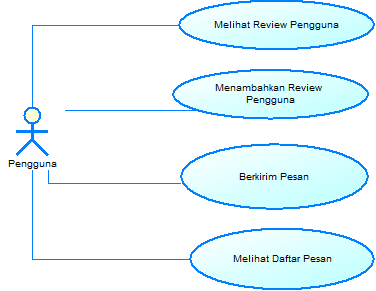
\includegraphics
		[width=\textwidth]
		{images/bab3/usecasediagram/ucd-04.png}
		\caption{Diagram Kasus Penggunaan Manajemen Interaksi Antarpengguna}
		\label{ucd.04}
	\end{figure}
Pada kasus penggunaan ini, pengguna difasilitasi untuk berinteraksi, memberikan \textit{review}/testimoni terhadap pengguna lainnya sesuai dengan keinginan.

	% Melihat review pengguna
	% Melihat review pengguna
	
\begin{table}[H]
	\centering
	\begin{tabular}{|r|p{8cm}|}
		\hline
		\textbf{Kode}                                                    
		& UC-04.01
		\\ \hline
		\textbf{Nama}                                                    
		& \textbf{Melihat \textit{Review} Pengguna} 
		\\ \hline
		
		\textbf{Aktor}  
		& Pengguna 
		\\ \hline
		
		\textbf{Deskripsi}
		& Pengguna ingin melihat \textit{review} pada pengguna tertentu
		\\ \hline
		\textbf{Tipe}                                                    
		& Fungsional 
		\\ \hline
		\textbf{\textit{Precondition}}
		& \textit{Review} pengguna belum ditampilkan
		\\ \hline
		\textbf{\textit{Postcondition}} 
		& \textit{Review} pengguna berhasil ditampilkan
		\\ \hline
		\multicolumn{2}{|c|}
		{\textbf{Alur Kejadian Normal}}                                                                            
		\\ \hline
		\multicolumn{1}{|l|}{} & 
		\begin{enumerate}
			% \item \label{uc0301-show1page}Sistem menampilkan halaman yang berisi form pendaftaran barang
			% \item \label{al-0301-a} Sistem memvalidasi data yang dimasukkan pengguna
			\item Pengguna mengklik \textit{link} profil pengguna
			\item \label{uc0401-a}Sistem menampilkan halaman profil pengguna
			\item Pengguna dapat melihat \textit{review} pengguna di bagian kiri bawah beserta rata-rata \textit{rating} yang diberikan.
		\end{enumerate}
		\\ \hline
		\multicolumn{2}{|c|}{\textbf{Alur Kejadian Alternatif}} \\ \hline
		\multicolumn{1}{|l|}{}                                           
		& -
		\\ \hline
	\end{tabular}
	\caption{Spesifikasi Kasus Penggunaan : Melihat \textit{Review} Pengguna}
	\label{uc04.01}
\end{table}

	
	% Menambahkan Review Pengguna
		% Menambahkan Review Pengguna
	
	
	\begin{table}[H]
		\centering
		\begin{tabular}{|r|p{8cm}|}
			\hline
			\textbf{Kode}                                                    
			& UC-04.02
			\\ \hline
			\textbf{Nama}                                                    
			& \textbf{ Menambahkan Review Pengguna } 
			\\ \hline
			\textbf{Aktor}                                                   
			& Pengguna 
			\\ \hline
			\textbf{Deskripsi}                                               
			& Pengguna ingin menambahkan review dari \textit{transaksi} yang pernah dilakukan.
			\\ \hline
			\textbf{Tipe}
			& Fungsional 
			\\ \hline
			
			\textbf{\textit{Precondition}}
			& Review dari pengguna belum tercatat/tersimpan dalam sistem

			\\ \hline
			
			\textbf{\textit{Postcondition}} 
			& Review dari pengguna berhasil tercatat dalam sistem
			\\ \hline
			
			\multicolumn{2}{|c|}
			{\textbf{Alur Kejadian Normal}}                                                                            
			\\ \hline
			\multicolumn{1}{|l|}{} & 
			\begin{enumerate}
				\item Pengguna mengklik halaman 'Riwayat Transaksi'
				\item Sistem menampilkan halaman Riwayat Transaksi yang pernah dilakukan pengguna
				\item Pengguna mengklik \textit{tab} jenis transaksi yang pernah dilakukan (Beli atau Lelang)
				\item \label{uc0402-show1page}Sistem menampilkan riwayat transaksi sesuai dengan jenis transaksi yang dipilih pengguna
				\item Pengguna mengklik transaksi yang ingin diberikan \textit{review}
				\item \label{al-0402-a}Sistem mengecek apakah \textit{review} sudah pernah diberikan sebelumnya
				\item Sistem menampilkan \textit{modal} berisi \textit{field input} jumlah \textit{rating}
				\item Pengguna mengisi \textit{field} tersebut sesuai jumlah rating yang ingin diberikan
				\item Setelah selesai, pengguna klik 'Next'
				\item Sistem menampilkan \textit{modal} kedua, berisikan \textit{field input} untuk deskripsi \textit{review}
				\item Pengguna mengisikan \textit{field input} sesuai dengan deskripsi yang ingin diberikan
				\item Setelah selesai, pengguna mengklik tombol 'Simpan Review'
				\item \label{al-0402-b}Sistem memvalidasi masukan dari pengguna
				\item Jika tervalidasi, sistem menampilkan modal berisi informasi sukses menyimpan review
				\item Pengguna klik tombol 'Oke'
				\item Sistem menutup \textit{modal} dan kembali ke halaman di poin \cref{uc0402-show1page}
				
				% \item \label{uc0301-show1page}Sistem menampilkan halaman yang berisi form pendaftaran barang
				% \item \label{al-0301-a} Sistem memvalidasi data yang dimasukkan pengguna
			\end{enumerate}
			\\ \hline
			\multicolumn{2}{|c|}{\textbf{Alur Kejadian Alternatif}} \\ \hline
			\multicolumn{1}{|l|}{}                                   \pagebreak        
			& \textbf{Review untuk transaksi yang dipilih sudah pernah diberikan}
			\\ \hline
			\multicolumn{1}{|l|}{}& 
			\begin{itemize}
				\item[\ref{al-0402-a}a.] Sistem mendeteksi bahwa review untuk transaksi tersebut sudah pernah dilakukan
				\item[\ref{al-0402-a}b.] Sistem menampilkan modal berisi informasi bahwa review sudah pernah diberikan, dan \textit{auto-close modal} setelah 4 detik
				\item[\ref{al-0402-a}c.] Sistem menampilkan halaman di poin \cref{uc0402-show1page}
			\end{itemize}
			\\ \hline
			
			\multicolumn{1}{|l|}{}      
			& \textbf{Data masukan pengguna tidak valid}
			\\ \hline
			\multicolumn{1}{|l|}{}& 
			\begin{itemize}
				\item[\ref{al-0402-b}a.] Sistem mendeteksi masukan pengguna tidak valid.
				\item[\ref{al-0402-b}b.] Sistem menampilkan pesan Error berisi \textit{error message}
				\item[\ref{al-0402-b}c.] Sistem menampilkan halaman di poin \cref{uc0402-show1page}
			\end{itemize}
			\\ \hline
		\end{tabular}
		\caption{Spesifikasi Kasus Penggunaan : Memberikan Review Pengguna}
		\label{uc0x.0x-tab}
	\end{table}
		
	% Berikirim pesan
		% Mengirim pesan
	
	
	\begin{table}[H]
		\centering
		\begin{tabular}{|r|p{8cm}|}
			\hline
			\textbf{Kode}
			& UC-04.04
			\\ \hline
			\textbf{Nama}
			& \textbf{ Mengirim Pesan } 
			\\ \hline
			\textbf{Aktor}    
			& Pengguna 
			\\ \hline
			\textbf{Deskripsi}
			& Pengguna akan mengirimkan pesan kepada pengguna lainnya
			\\ \hline
			\textbf{Tipe}
			& Fungsional 
			\\ \hline
			\textbf{\textit{Precondition}}
			& Pesan yang dikirimkan pengguna belum tersimpan pada sistem
			\\ \hline
			\textbf{\textit{Postcondition}} 
			& Pesan yang dikirimkan pengguna berhasil tersimpan pada sistem
			\\ \hline
			\multicolumn{2}{|c|}
			{\textbf{Alur Kejadian Normal}}
			\\ \hline
			\multicolumn{1}{|l|}{} & 
			\begin{enumerate}
				\item Pengguna mengklik \textit{URL} pengguna tujuan yang ingin dikirimi pesan
				\item Sistem menampilkan halaman profil pengguna tujuan
				\item Pengguna mengklik tombol "Kirim Pesan"
				\item Sistem menampilkan halaman percakapan pengguna terhadap tujuan beserta riwayat percakapan pengguna dengan pengguna tujuan
				\item \label{al-0404-ex} Pengguna memasukkan pesan yang ingin dikirimkan pada \textit{field input} yang disediakan
				\item Setelah selesai, pengguna mengklik tombol 'Kirim'
				\item \label{al-0404-a}Sistem mengirim kepada koneksi soket
				\item Jika proses pengiriman kepada soket berhasil dan tidak ada gangguan, sistem kembali menampilkan halaman pengguna dengan informasi pesan yang sudah terkirim muncul di riwayat percakapan pengguna dengan pengguna tujuan
				
				% \item \label{uc0301-show1page}Sistem menampilkan halaman yang berisi form pendaftaran barang
				% \item \label{al-0301-a} Sistem memvalidasi data yang dimasukkan pengguna
			\end{enumerate}
			\\ \hline
			\multicolumn{2}{|c|}{\textbf{Alur Kejadian Alternatif}} \\ \hline
			\multicolumn{1}{|l|}{}                   
			& \textbf{Terjadi masalah teknis sehingga pesan tidak dapat terkirim}
			\\ \hline
			\multicolumn{1}{|l|}{}& 
			\begin{itemize}
				\item[\ref{al-0404-a}a.] Sistem mendapatkan \textit{exception} dari koneksi soket, bahwa pesan tidak dapat tersimpan
				\item[\ref{al-0404-a}b.] Sistem menampilkan kembali halaman pada poin \ref{al-0404-ex}, dengan \textit{modal} berisikan \textit{error message}
			\end{itemize}
			\\ \hline
		\end{tabular}
		\caption{Spesifikasi Kasus Penggunaan : Mengirimkan Pesan}
		\label{uc04.04-tab}
	\end{table}

	% Melihat daftar pesan
		% Melihat dan membaca pesan
	
	
	\begin{table}[H]
		\centering
		\begin{tabular}{|r|p{8cm}|}
			\hline
			\textbf{Kode}
			& UC-04.05
			\\ \hline
			\textbf{Nama}
			& \textbf{Melihat daftar Pesan} 
			\\ \hline
			\textbf{Aktor}    
			& Pengguna 
			\\ \hline
			\textbf{Deskripsi}
			& Pengguna ingin melihat daftar percakapan/ daftar perpesanan yang pernah dilakukan pengguna
			\\ \hline
			\textbf{Tipe}
			& Fungsional 
			\\ \hline
			\textbf{\textit{Precondition}}
			& Daftar percakapan/ daftar perpesanan belum ditampilkan
			\\ \hline
			\textbf{\textit{Postcondition}} 
			& Daftar percakapan/ daftar perpesanan berhasil ditampilkan
			\\ \hline
			\multicolumn{2}{|c|}
			{\textbf{Alur Kejadian Normal}}
			\\ \hline
			\multicolumn{1}{|l|}{} & 
			\begin{enumerate}
				\item Pengguna mengklik tombol 'Conversations' di \textit{navbar} aplikasi
				\item \label{al-0405-a} Sistem menampilkan halaman daftar percakapan pengguna
				\item Sistem memanggil fungsi AJAX untuk meminta data-data percakapan terakhir pengguna
				\item Balasan dari fungsi AJAX di \textit{load} oleh \textit{browser} untuk selanjutnya di\textit{parse} ke dalam HTML
				\item Sistem menampilkan daftar percakapan pengguna
				\item Pengguna mengklik percakapan yang ingin dilihat/dibaca
				\item Sistem menampilkan detail percakapan pengguna dengan pengguna tujuan
			\end{enumerate}
			\\ \hline
		\end{tabular}
		\caption{Spesifikasi Kasus Penggunaan: Melihat \& Membaca Pesan}
		\label{uc04.05}
	\end{table}
	
%	\subsubsection{KP05. \textit{Monitoring} Proses Lelang}
\label{kp05}
	\begin{figure}[H]
		\centering
		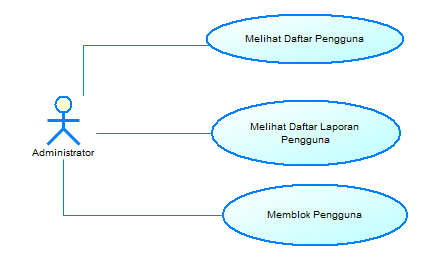
\includegraphics
		[width=\textwidth]
		{images/bab3/buku/usecasediagram/ucd-05.png}
		\caption{Diagram Kasus Penggunaan \textit{Monitoring} Lelang}
		\label{ucd.05}
	\end{figure}
Kasus penggunaan ini seluruhnya digunakan oleh \textit{administrator} aplikasi, dan dilakukan di sistem terpisah.

% Melihat daftar pengguna
	% 
	
	
	\begin{table}[H]
		\centering
		\begin{tabular}{|r|p{8cm}|}
			\hline
			\textbf{Kode}                                                    
			& UC-04.02
			\\ \hline
			\textbf{Nama}                                                    
			& \textbf{ Menambahkan \textit{Review} Pengguna } 
			\\ \hline
			\textbf{Aktor}                                                   
			& Pengguna 
			\\ \hline
			\textbf{Deskripsi}                                               
			& Pengguna ingin menambahkan \textit{review} dari \textit{transaksi} yang pernah dilakukan.
			\\ \hline
			\textbf{Tipe}
			& Fungsional 
			\\ \hline
			
			\textbf{\textit{Precondition}}
			& \textit{Review} dari pengguna belum tercatat/tersimpan dalam sistem

			\\ \hline
			
			\textbf{\textit{Postcondition}} 
			& \textit{Review} dari pengguna berhasil tercatat dalam sistem
			\\ \hline
			
			\multicolumn{2}{|c|}
			{\textbf{Alur Kejadian Normal}}                                                                            
			\\ \hline
			\multicolumn{1}{|l|}{} & 
			\begin{enumerate}
				\item Pengguna mengklik halaman 'Riwayat Transaksi'
				\item Sistem menampilkan halaman Riwayat Transaksi yang pernah dilakukan pengguna
				\item Pengguna mengklik \textit{tab} jenis transaksi yang pernah dilakukan (Beli atau Lelang)
				\item \label{uc0402-show1page}Sistem menampilkan riwayat transaksi sesuai dengan jenis transaksi yang dipilih pengguna
				\item Pengguna mengklik transaksi yang ingin diberikan \textit{review}
				\item \label{al-0402-a}Sistem mengecek apakah \textit{review} sudah pernah diberikan sebelumnya
				\item Sistem menampilkan \textit{modal} berisi \textit{field input} jumlah \textit{rating}
				\item Pengguna mengisi \textit{field} tersebut sesuai jumlah rating yang ingin diberikan
				\item Setelah selesai, pengguna klik 'Next'
				\item Sistem menampilkan \textit{modal} kedua, berisikan \textit{field input} untuk deskripsi \textit{review}
				\item Pengguna mengisikan \textit{field input} sesuai dengan deskripsi yang ingin diberikan
				\item Setelah selesai, pengguna mengklik tombol 'Simpan Review'
				\item \label{al-0402-b}Sistem memvalidasi masukan dari pengguna
				\item Jika tervalidasi, sistem menampilkan modal berisi informasi sukses menyimpan review
				\item Pengguna klik tombol 'Oke'
				\item Sistem menutup \textit{modal} dan kembali ke halaman di poin \ref{uc0402-show1page}
				
				% \item \label{uc0301-show1page}Sistem menampilkan halaman yang berisi form pendaftaran barang
				% \item \label{al-0301-a} Sistem memvalidasi data yang dimasukkan pengguna
			\end{enumerate}
			\\ \hline
			\multicolumn{2}{|c|}{\textbf{Alur Kejadian Alternatif}} \\ \hline
			\multicolumn{1}{|l|}{}                                   \pagebreak        
			& \textbf{Review untuk transaksi yang dipilih sudah pernah diberikan}
			\\ \hline
			\multicolumn{1}{|l|}{}& 
			\begin{itemize}
				\item[\ref{al-0402-a}a.] Sistem mendeteksi bahwa review untuk transaksi tersebut sudah pernah dilakukan
				\item[\ref{al-0402-a}b.] Sistem menampilkan modal berisi informasi bahwa review sudah pernah diberikan, dan \textit{auto-close modal} setelah 4 detik
				\item[\ref{al-0402-a}c.] Sistem menampilkan halaman di poin \ref{uc0402-show1page}
			\end{itemize}
			\\ \hline
			
			\multicolumn{1}{|l|}{}      
			& \textbf{Data masukan pengguna tidak valid}
			\\ \hline
			\multicolumn{1}{|l|}{}& 
			\begin{itemize}
				\item[\ref{al-0402-b}a.] Sistem mendeteksi masukan pengguna tidak valid.
				\item[\ref{al-0402-b}b.] Sistem menampilkan pesan Error berisi \textit{error message}
				\item[\ref{al-0402-b}c.] Sistem menampilkan halaman di poin \ref{uc0402-show1page}
			\end{itemize}
			\\ \hline
		\end{tabular}
		\caption{Spesifikasi Kasus Penggunaan : Memberikan \textit{Review} Pengguna}
		\label{uc04.02}
	\end{table}

% Melihat daftar laporan pengguna
	% Menambahkan Review Pengguna
	
	
	\begin{table}[H]
		\centering
		\caption{Spesifikasi Kasus Penggunaan : Memberikan \textit{Review} Pengguna}
		\label{uc04.02}
		\begin{tabular}{|r|p{8cm}|}
			\hline
			\textbf{Kode}                                                    
			& UC-04.02
			\\ \hline
			\textbf{Nama}                                                    
			& \textbf{ Menambahkan \textit{Review} Pengguna } 
			\\ \hline
			\textbf{Aktor}                                                   
			& Pengguna 
			\\ \hline
			\textbf{Deskripsi}                                               
			& Pengguna ingin menambahkan \textit{review} dari \textit{transaksi} yang pernah dilakukan.
			\\ \hline
			\textbf{Tipe}
			& Fungsional 
			\\ \hline
			
			\textbf{\textit{Precondition}}
			& \textit{Review} dari pengguna belum tercatat/tersimpan dalam sistem \\ \hline
			
			\textbf{\textit{Postcondition}} 
			& \textit{Review} dari pengguna berhasil tercatat dalam sistem
			\\ \hline
			
			\multicolumn{2}{|c|}
			{\textbf{Alur Kejadian Normal}}                                                                            
			\\ \hline
			\multicolumn{1}{|l|}{} & 
			\begin{enumerate}
				\item Pengguna mengklik halaman 'Riwayat Transaksi'
				\item Sistem menampilkan halaman Riwayat Transaksi yang pernah dilakukan pengguna
				\item Pengguna mengklik \textit{tab} jenis transaksi yang pernah dilakukan (Beli atau Lelang)
				\item \label{uc0402-show1page}Sistem menampilkan riwayat transaksi sesuai dengan jenis transaksi yang dipilih pengguna
				\item Pengguna mengklik transaksi yang ingin diberikan \textit{review}
				\item \label{al-0402-a}Sistem mengecek apakah \textit{review} sudah pernah diberikan sebelumnya, lalu menampilkan form penilaian selanjutnya.
				\item Pengguna memasukkan jumlah \textit{rating} dan deskripsi \textit{rating}, lalu klik 'Simpan Review'
				\item \label{al-0402-b}Sistem memvalidasi masukan, jika valid sistem mengembalikan modal status sukses.				
				% \item \label{uc0301-show1page}Sistem menampilkan halaman yang berisi form pendaftaran barang
				% \item \label{al-0301-a} Sistem memvalidasi data yang dimasukkan pengguna
			\end{enumerate}
			\\ \hline
			\multicolumn{2}{|c|}{\textbf{Alur Kejadian Alternatif}} \\ \hline
			\multicolumn{1}{|l|}{}                                   \pagebreak        
			& -
			\\ \hline
		\end{tabular}
	\end{table}

% Memblock pengguna
	% Melaporkan Barang
	
	
	\begin{table}[H]
		\centering
		\begin{tabular}{|r|p{8cm}|}
			\hline
			\textbf{Kode}                                                    
			& UC-04.03
			\\ \hline
			\textbf{Nama}
			
			& \textbf{Melaporkan Barang} 
			\\ \hline
			\textbf{Aktor}                                                   
			& Pengguna 
			\\ \hline
			\textbf{Deskripsi}                                               
			& Pengguna ingin melaporkan barang yang dianggap melanggar aturan/tidak pantas diperjualbelikan
			\\ \hline
			\textbf{Tipe}                                                    
			& Fungsional 
			\\ \hline
			\textbf{\textit{Precondition}}
			& Laporan dari pengguna belum tersimpan dalam sistem
			\\ \hline
			\textbf{\textit{Postcondition}} 
			& Laporan dari pengguna berhasil tersimpan dalam sistem
			\\ \hline
			\multicolumn{2}{|c|}
			{\textbf{Alur Kejadian Normal}}                                                                            
			\\ \hline
			\multicolumn{1}{|l|}{} & 
			\begin{enumerate}
				\item Pengguna mengklik barang yang ingin dilaporkan
				\item \label{uc0403-1page} Sistem menampilkan halaman informasi barang
				\item Pengguna mengklik tombol "Laporkan Barang"
				\item Sistem menampilkan \textit{modal} berisi \textit{input field} laporan
				\item Pengguna mengisi \textit{fields} tersebut sesuai dengan konten laporan yang ingin disampaikan
				\item \label{uc0403-modal}Setelah selesai, pengguna mengklik tombol "Laporkan"
				\item Sistem mengecek dan memvalidasi masukan pengguna
				\item Jika valid, sistem akan menampilkan \textit{modal} Sukses Menyimpan Laporan
				\item Sistem me\textit{redirect} pengguna kembali ke halaman di \ref{uc0403-1page}
				% \item \label{uc0301-show1page}Sistem menampilkan halaman yang berisi form pendaftaran barang
				% \item \label{al-0301-a} Sistem memvalidasi data yang dimasukkan pengguna
			\end{enumerate}
			\\ \hline
			\multicolumn{2}{|c|}{\textbf{Alur Kejadian Alternatif}} \\ \hline
			\multicolumn{1}{|l|}{}      
			& \textbf{Data masukan laporan pengguna tidak valid}
			\\ \hline
			\multicolumn{1}{|l|}{}& 
			\begin{itemize}
				\item[\ref{al-0402-b}a.] Sistem mendeteksi masukan pengguna tidak valid.
				\item[\ref{al-0402-b}c.] Sistem menampilkan kembali modal di poin \ref{uc0403-modal} beserta dengan \textit{error message}
			\end{itemize}
			\\ \hline
		\end{tabular}
		\caption{Spesifikasi Kasus Penggunaan : Melaporkan Barang}
		\label{uc04.03-tab}
	\end{table}
	
	\subsubsection{KP05. Manajemen Voucher}
\label{kp05}

	\begin{figure}[H]
		\centering
		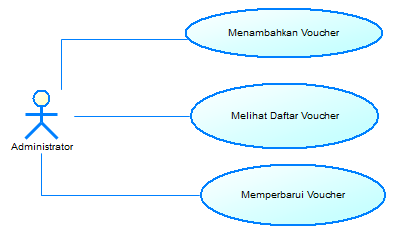
\includegraphics
		[width=\textwidth]
		{images/bab3/usecasediagram/ucd-06.png}
		\caption{Diagram Kasus Penggunaan Manajemen Kupon}
		\label{ucd.06}
	\end{figure}
	Kasus penggunaan ini seluruhnya digunakan oleh \textit{administrator} aplikasi dan dilakukan di sistem terpisah. Kasus penggunaan ditujukan untuk mempermudah \textit{administrator} dalam memanajemen voucher/kupon yang dibagikan oleh pengguna.

	% Menambahkan voucher
		% Memasukkan kupon
	
	\begin{table}[H]
		\centering
		\begin{tabular}{|r|p{8cm}|}
			\hline
			\textbf{Kode}
			& UC-05.01
			\\ \hline
			\textbf{Nama}
			& \textbf{Menambahkan Kupon} 
			\\ \hline
			\textbf{Aktor}    
			& Administrator 
			\\ \hline
			\textbf{Deskripsi}
			& Administrator ingin menggunakan kupon/voucher yang ia miliki untuk pada sebuah transaksi
			\\ \hline
			\textbf{Tipe}
			& Fungsional 
			\\ \hline
			\textbf{\textit{Precondition}}
			& Kupon baru belum berhasil tersimpan di sistem
			\\ \hline
			\textbf{\textit{Postcondition}} 
			& Kupon baru berhasil tersimpan di sistem
			\\ \hline
			\multicolumn{2}{|c|}
			{\textbf{Alur Kejadian Normal}}
			\\ \hline
			\multicolumn{1}{|l|}{} & 
			\begin{enumerate}
				\item Administrator membuka halaman 'Tambah Kupon'
				\item Sistem menampilkan halaman form Tambah Kupon
				\item Administrator memasukkan informasi kupon baru yang akan ditambahkan
				\item Sistem mengecek permintaan penggunaan kupon,jika permintaan dapat diverifikasi dan valid, sistem me\textit{redirect} ke halaman manajemen kupon.
				% \item \label{uc0301-show1page}Sistem menampilkan halaman yang berisi form pendaftaran barang
				% \item \label{al-0301-a} Sistem memvalidasi data yang dimasukkan pengguna
			\end{enumerate}
			\\ \hline
			\multicolumn{2}{|c|}{\textbf{Alur Kejadian Alternatif}} \\ \hline
			\multicolumn{1}{|l|}{}                   
			& -
			\\ \hline
		\end{tabular}
		\caption{Spesifikasi Kasus Penggunaan : Menambahkan Kupon}
		\label{uc06.01}
	\end{table}
	
	% Melihat daftar voucher
		% Memasukkan kupon
	
	\begin{table}[H]
		\centering
		\begin{tabular}{|r|p{8cm}|}
			\hline
			\textbf{Kode}
			& UC-05.02
			\\ \hline
			\textbf{Nama}
			& \textbf{Memasukkan Kupon pada Transaksi} 
			\\ \hline
			\textbf{Aktor}    
			& Pengguna 
			\\ \hline
			\textbf{Deskripsi}
			& Pengguna ingin menggunakan kupon/voucher yang ia miliki untuk pada sebuah transaksi
			\\ \hline
			\textbf{Tipe}
			& Fungsional 
			\\ \hline
			\textbf{\textit{Precondition}}
			& Pengguna belum berhasil men\textit{submit} kode kupon ke dalam transaksi barang
			\\ \hline
			\textbf{\textit{Postcondition}} 
			& Pengguna berhasil men\textit{submit} kode kupon ke dalam transaksi barang
			\\ \hline
			\multicolumn{2}{|c|}
			{\textbf{Alur Kejadian Normal}}
			\\ \hline
			\multicolumn{1}{|l|}{} & 
			\begin{enumerate}
				\item Pengguna membuka halaman 'Riwayat Transaksi Lelang'
				\item Sistem menampilkan halaman Riwayat Transaksi Lelang pengguna
				\item Pengguna mengklik tombol 'Masukkan Kupon' pada transaksi yang diinginkan
				\item Sistem mengecek permintaan penggunaan kupon
				\item Jika permintaan dapat diverifikasi dan valid, sistem menampilkan \textit{modal} berisi \textit{input field} kupon
				\item Pengguna memasukkan kupon yang ingin dimasukkan, lalu mengklik tombol 'Submit'
				\item Sistem memvalidasi kupon voucher dan status barang
				\item Jika valid, sistem menerapkan penggunaan kupon ke dalam transaksi barang
				\item Sistem lalu menampilkan \textit{modal} yang berisi informasi sukses penggunaan kupon pada transaksi
				% \item \label{uc0301-show1page}Sistem menampilkan halaman yang berisi form pendaftaran barang
				% \item \label{al-0301-a} Sistem memvalidasi data yang dimasukkan pengguna
			\end{enumerate}
			\\ \hline
			\multicolumn{2}{|c|}{\textbf{Alur Kejadian Alternatif}} \\ \hline
			\multicolumn{1}{|l|}{}                   
			& -
			\\ \hline
		\end{tabular}
		\caption{Spesifikasi Kasus Penggunaan : Mendaftarkan Barang Lelang}
		\label{uc04.06}
	\end{table}
	
	% Memperbarui Voucher
		% Memasukkan kupon
	
	\begin{table}[H]
		\centering
		\begin{tabular}{|r|p{8cm}|}
			\hline
			\textbf{Kode}
			& UC-05.01
			\\ \hline
			\textbf{Nama}
			& \textbf{Memperbarui Kupon} 
			\\ \hline
			\textbf{Aktor}    
			& Administrator 
			\\ \hline
			\textbf{Deskripsi}
			& Administrator ingin memperbarui kupon
			\\ \hline
			\textbf{Tipe}
			& Fungsional 
			\\ \hline
			\textbf{\textit{Precondition}}
			& Kupon belum diperbarui
			\\ \hline
			\textbf{\textit{Postcondition}} 
			& Kupon berhasil diperbarui
			\\ \hline
			\multicolumn{2}{|c|}
			{\textbf{Alur Kejadian Normal}}
			\\ \hline
			\multicolumn{1}{|l|}{} & 
			\begin{enumerate}
				\item Administrator membuka halaman 'Manajemen Kupon'
				\item Sistem menampilkan halaman form Edit Kupon pada sesuai dengan data kupon yang ingin diperbarui
				\item Administrator memasukkan informasi kupon baru yang ingin ditambahkan, lalu ketik tombol "Submit"
				\item Sistem mengecek informasi baru kupon kupon,lalu sistem me\textit{redirect} ke halaman manajemen kupon dengan info sukses.
				% \item \label{uc0301-show1page}Sistem menampilkan halaman yang berisi form pendaftaran barang
				% \item \label{al-0301-a} Sistem memvalidasi data yang dimasukkan pengguna
			\end{enumerate}
			\\ \hline
			\multicolumn{2}{|c|}{\textbf{Alur Kejadian Alternatif}} \\ \hline
			\multicolumn{1}{|l|}{}                   
			& -
			\\ \hline
		\end{tabular}
		\caption{Spesifikasi Kasus Penggunaan : Menambahkan Kupon}
		\label{uc06.03}
	\end{table}







 %checked
	%Technical Analysis


	\subsection{\textit{Technical Analysis}}
	\label{tech-analysis}
	
	Untuk membuat sebuah aplikasi yang sukses, tentunya banyak sekali aspek yang harus diperhatikan. Selain kualitas aplikasi yang akan dibuat, juga ketahanannya terhadap perubahan karena \textit{e-commerce} adalah sesuatu yang sangat cepat berubah karena kompetitor yang sangat kompetitif dan dorongan tehnologi yang membuat efektifitas dan efisiensi menjadi lebih baik.\\
	
	\indent Dari sisi \textit{software engineering} sendiri, \textit{software engineering} dimaksudkan untuk menunjang/\textit{support} pengembangan \textit{software} daripada \textit{individual programming}. Hal ini mencakup: \begin{inlinelist}
		\item \textit{evolution}
		\item \textit{design}
		\item \textit{supporting program specification}
	\end{inlinelist} \cite[p.~5]{software-engineering}
	
	\begin{figure}[H]
		\centering
		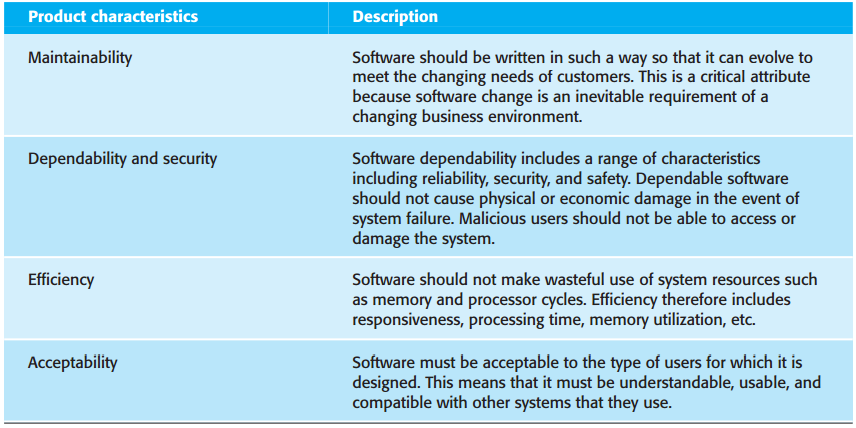
\includegraphics[width=.8\textwidth]{images/bab3/buku/essential-good-software.png}
		\caption{\textit{Essential attributes of good software}}
		\label{essential-software}
	\end{figure}
	
	\indent Berdasarkan kriteria tersebut, maka setiap poin perlu diperhatikan agar dapat mengembangkan sebuah aplikasi yang tidak hanya sukses, tapi juga bertahan dalam kompetisi. Dalam istilah bisnis, hal ini disebut dengan \textit{risk management}.
	
	% pemaparan evolution-risk from inside : data growth, latency
	
	% pemaparan evolution-risk from outside : keamanan
	% pemaparan gabungan 	
	
\subsection{Analisa Penulis}
	\subsubsection{Analisa \textit{User Experience} dari E-Commerce di Indonesia}
	\label{alasan-ux-ecommerce-indonesia alasan-app-serupa}
	Selama masa pengerjaan aplikasi, penulis sering menganalisa dan memperhatikan kebiasaan-kebiasaan yang umum di website \textit{e-commerce} di Indonesia. Salah satu yang paling sering dianalisa oleh penulis adalah adalah situs Tokopedia. Dalam pengembangannya, \textit{user interface} aplikasi akan dipengaruhi analisa ini, yang dijabarkan seperti berikut:
	\begin{enumerate}
		\item Halaman yang muncul bukanlah eagerloading, tapi \textit{lazy loading}\\
		\indent Ini adalah solusi cerdas untuk mengakali \textit{delay loading item} yang sudah pasti jumlahnya sangat banyak (maka butuh \textit{query} yang tentunya memakan waktu cukup lama), namun juga memainkan faktor psikologi / \textit{user behaviour} pengguna dengan membiarkan pengguna melihat tahap demi tahap halaman 'diisi'.
		\item \textit{User Interface} yang sederhana dan pemilihan warna yang \textit{soft}
	\end{enumerate}
	
	\subsubsection{Analisa Keamanan pada koneksi Soket}
	\label{alasan-socket.io}
	Untuk mengakomodasi fitur yang bersifat \textit{realtime}, dibutuhkan koneksi ke soket secara terus menerus. Hal ini tentu dapat menjadi sasaran empuk \textit{security} karena jika tidak diamankan, maka dapat menjadi peluang besar bagi para pihak yang tidak berkepentingan untuk merusak proses bisnis aplikasi.\\
	\indent Namun, jika dalam setiap koneksi soket harus mengirimkan \textit{credentials}, hal ini tentu menjadi tidak praktis dan malah lebih berbahaya karena membiarkan data-data sensitif seperti \textit{password} dan \textit{username} berlalu-lalang di jaringan internet. Selain itu, \textit{disadvantage}nya adalah ketidakpraktisan untuk selalu meng\textit{query} database setiap kali ada koneksi, tentu saja ini memperlambat kerja \textit{database} dan menambah waktu \textit{delay}. Maka dari itu, penulis mengidentifikasi poin-poin penting berikut :
		\begin{itemize}
			\item Hindari \textit{query} database untuk \textit{autentikasi} yang sifatnya masif
			\item Menggunakan mekanisme authentikasi yang menggunakan \textit{credentials} karena rentan dengan masalah keamanan
			\item Mencari metode yang lebih efektif, cepat untuk autentikasi selain 
		\end{itemize}
	
	\subsubsection{Analisa \textit{Best Practice} dalam Struktur Perangkat Lunak}
		\label{alasan-best-practice}
		Pada dasarnya, Laravel adalah kerangka kerja MVC. Namun, ada banyak fitur yang ada dalam aplikasi Lelang Online ini yang tidak terakomodasi dalam MVC, misal sebagai berikut :
		\begin{enumerate}
			\item Sistem Verifikasi lewat Email - yang berarti aplikasi harus berinteraksi dengan SMTP server
			\item Sistem \textit{Generate} Token JWT.io, dimana dalam proses \textit{Generate Token} sama sekali tidak ada database dilibatkan.
		\end{enumerate}
		\indent Jika fitur-fitur tersebut 'dipaksa' dimuat ke dalam MVC, maka tentu saja strukturnya menjadi ganjil, dan muncul \textit{code smell} berikut :
		\begin{enumerate}
			\item \textit{Large Class}, dimana terdapat satu buah file yang sangat panjang (biasanya merupakan entitas utama, dalam hal ini contohnya barang/\textit{item})
			\item \textit{Inappropriate Intimacy}, dimana terdapat satu kelas yang menyimpan \textit{logic} yang tidak seharusnya ia simpan
			\item \textit{Duplicated Code}
		\end{enumerate}		
		\indent Dari hasil analisa ini, penulis mengidentifikasikan strategi-strategi yang akan diterapkan dalam rancangan struktur aplikasi pada subbab \ref{software-structure}, yaitu sebagai berikut:
			\begin{enumerate}
				\item Penggunaan Repository Pattern
				\\ Memisahkan antara Data Processing Layer dan View Layer - agar lebih rapi, terstruktur, hal ini juga dapat menghindari \textit{Duplicated Code}.
				\item Penambahan Komponen : Service dan Provider \\
				Untuk memisahkan \textit{logic} aplikasi yang terkait dengan akses\textit{eksternal services}. Tujuannya, agar jika kedepannya terdapat perbaikan fitur/penambahan fitur, lebih mudah melakukan \textit{traceback} terhadap file/kelas yang bertanggungjawab terhadap fitur tersebut.
			\end{enumerate}
	
	\subsubsection{Analisa Aplikasi Serupa}
	\label{alasan-app-serupa}
		Selama pengerjaan aplikasi, penulis menganalisa aplikasi serupa. Penulis menemukan aplikasi yang kurang lebih alur bisnis/alur penggunaan aplikasinya serupa yaitu : Carousell. Penulis melihat beberapa kesamaan antara sifat transaksi aplikasi tugas akhir saya dengan aplikasi tersebut, yaitu:
		\begin{enumerate}
			\item Sama-sama tidak mengakomodasi pembayaran
			\item Sama-sama tidak adanya kepastian harga (bedanya, pada Carousell yang terjadi adalah \textit{bargaining}
		\end{enumerate} \
		\indent Sehingga dalam alur proses nya, banyak diadaptasi dari Carousell, agar pengguna dapat lebih familiar dan \textit{predictability}nya lebih tinggi jika diadaptasi dari \textit{E-commerce} lainnya yang lebih umum digunakan oleh pengguna.
		
	
	\subsubsection{Analisa Aplikasi Serupa}
	\label{alasan-app-serupa}
	Selama pengerjaan aplikasi, penulis menganalisa aplikasi serupa. Penulis menemukan aplikasi yang kurang lebih alur bisnis / alur penggunaan aplikasinya serupa yaitu : Carousell. \\
	\indent Penulis melihat ada beberapa kesamaan antara sifat transaksi aplikasi tugas akhir saya dengan aplikasi tersebut, yaitu :
	\begin{enumerate}
		\item Sama-sama tidak mengakomodasi pembayaran
		\item Sama-sama tidak adanya kepastian harga (bedanya, pada Carousell yang terjadi adalah \textit{bargaining}
	\end{enumerate}
	\indent Sehingga dalam alur proses nya, banyak diadaptasi dari Carousell, agar pengguna dapat lebih familiar dan \textit{predictability}nya lebih tinggi jika diadaptasi dari \textit{E-commerce} lainnya yang lebih umum digunakan oleh pengguna.
	
	\subsubsection{Analisa Penyimpanan Data}
	
	Untuk penyimpanan data, terdapat 2 jenis data yang sifatnya cukup berbeda, yaitu sebagai berikut:
	\begin{enumerate}
		\item \textbf{Data transaksional disimpan di DBMS SQL - \textit{Relational}}
		\newline
		\indent Data yang sifatnya \textit{transaksional}, seperti data \textit{bidding}, data pengguna, dan lain sebagainya.
		Untuk data ini, lebih baik jika menggunakan database Postgre, untuk menjaga integritas data dan \textit{integrity checking} juga  menjadi lebih baik.
		\item \textbf{Data non-transaksional disimpan di DBMS NoSQL}
		\newline
		\indent Data \textit{chatting}, data \textit{joined rooms} kurang tepat jika disimpan dalam database transaksional karena sifat pertambahan datanya yang sangat cepat, masif dan urgensi integritas data tidak terlalu diprioritaskan (dibanding dengan data transaksional pada poin sebelumnya). Oleh karena itu, baiknya data ini disimpan pada database NoSQL dengan alasan-alasan sebagai berikut.
		\begin{itemize} 
			\item Banyaknya transaksi \textit{read write};
			\item Ketidaksamaan frekuensi \textit{read and write} data semua pengguna;
			\item Sifat permintaan transaksi yang cepat; dan
			\item Kemungkinan perubahan struktur atribut pada pesan (misal: \textit{attachments}, \textit{forwarding}, \textit{replying}, dll) akan sangat menyulitkan pengembangan selanjutnya jika menggunakan database transaksional yang terpaku pada skema database yang ditetapkan di awal pengembangan aplikasi.
		\end{itemize} 	
		
		\item \textbf{Data citra/gambar menggunakan layanan Pihak Ketiga} \newline
		\indent Sekarang telah banyak penyedia jasa \textit{cloud computing} sebagai infrastruktur, seperti Amazon Web Service, Google Cloud Storage Google Alasan-alasan menggunakan AWS sebagai data storage untuk gambar adalah sebagai berikut :
		\begin{enumerate}[noitemsep,topsep=0pt]
			\item Skalabilitas aplikasi lebih terjaga. 
			\newline Dengan memisahkan penyimpanan antara gambar dan server sehingga lebih mudah me\textit{maintain} perkembangan aplikasi, dan lebih fokus terhadap pengembangan aplikasi.
			\item Menyediakan \textit{built-in} keamanan, fleksibel dan efisiensi \cite{wikipedia_amazon_2016}
		\end{enumerate}
		
		\item \textbf{Optimasi \textit{assets}} \newline
		\indent Dalam banyak kesempatan, penulis seringkali mendapati bahwa \textit{delay} untuk \textit{loading assets} lebih lama daripada \textit{loading data} dari database. Berikut penulis akan memaparkan hasil analisa berupa penyebab dan \textit{tackling} permasalahan tersebut.
			\begin{enumerate}
				\item \textit{Useless assets} yang disertakan dalam halaman: Memisahkan \textit{essentials assets} dan menyertakan \textit{script} yang hanya digunakan oleh halaman tersebut.
				\item Logika penyusunan script yang tidak efektif dan optimal (misal: ada satu script yang menyertakan file yang tidak diperlukan): \textit{pre-processing} berupa \textit{minifying, optimization, compiling, compression} terhadap \textit{assets}
				\item Latensi ke \textit{server} yang cukup tinggi (misal: kecepatan sambungan internet yang rendah): \textit{Caching}, \textit{upgrading server} agar dapat "lebih terjangkau" secara jaringan, penerapan PWA (\textit{Progressive Web Apps}) untuk sisi \textit{user experience}.
			\end{enumerate}
	\end{enumerate} %doneded
	
	
